% PLANTILLA APA7
% Creado por: Isaac Palma Medina
% Última actualización: 25/07/2021
% @COPYLEFT

% Fuentes consultadas (todos los derechos reservados):  
% Normas APA. (2019). Guía Normas APA. https://normas-apa.org/wp-content/uploads/Guia-Normas-APA-7ma-edicion.pdf
% Tecnológico de Costa Rica [Richmond]. (2020, 16 abril). LaTeX desde cero con Overleaf (1 de 3) [Vídeo]. YouTube. https://www.youtube.com/watch?v=kM1KvHVuaTY Weiss, D. (2021). 
% Formatting documents in APA style (7th Edition) with the apa7 LATEX class. https://ctan.math.washington.edu/tex-archive/macros/latex/contrib/apa7/apa7.pdf @COPYLEFT

%+-+-+-+-++-+-+-+-+-+-+-+-+-++-+-+-+-+-+-+-+-+-+-+-+-+-+-+-+-+-++-+-+-+-+-+-+-+-+-+

% Preámbulo
\documentclass[stu, 11pt, letterpaper, donotrepeattitle, floatsintext, natbib, helv]{apa7}
\usepackage{lipsum}
\usepackage[utf8]{inputenc}
\usepackage{comment}
\usepackage{marvosym}
\usepackage{graphicx}
\usepackage{float}
\usepackage[normalem]{ulem}
\usepackage[spanish]{babel} 
\usepackage{titling}
\usepackage{algpseudocode}
\usepackage{algorithm}
\usepackage{wrapfig}
\usepackage{tikz}
\usetikzlibrary{positioning,matrix, arrows.meta, backgrounds}
\usetikzlibrary{matrix,backgrounds}
\usepackage{subfigure}
\makeatletter
\renewcommand{\ALG@name}{Algoritmo}
\makeatother
\usepackage{setspace}
\usepackage{titling}
\let\apasubparagraph\subparagraph
\let\subparagraph\paragraph
\usepackage[compact]{titlesec}
\let\subparagraph\apasubparagraph
\usepackage{hyperref}
\selectlanguage{spanish}
\useunder{\uline}{\ul}{}
\newcommand{\myparagraph}[1]{\paragraph{#1}\mbox{}\\}
\graphicspath{{./images/}}

\titleformat{\part}{\normalfont\LARGE\bfseries}{\thetitle. \quad }{0pt}{}[{ \titlerule[0.8pt]}]
\titleformat{\section}{\normalfont\large\bfseries}{\thetitle. \quad }{0pt}{}[{ \titlerule[0.8pt]}]
\titleformat{\subsection}{\normalfont\bfseries}{}{}{}[]

\renewenvironment{abstract}{%
    \small
    \begin{center}%
        {\bfseries \abstractname\vspace{-.5em}\vspace{0pt}}%
    \end{center}%
    \quotation
    }
{\endquotation}

% \providecommand{\keywords}[1]
% {
%   \small	
%   \textbf{\textit{Palabras Clave---}} #1
% }
% Portada




% Palabras claves
\begin{document}
\title{\LARGE Sobre Matching en Hileras}
\author{\large Victor David Coto Solano \vskip0.3ex Diego Quirós Artiñano \vskip0.3ex Derek Rojas Mendoza} % (autores separados, consultar al docente)
% Manera oficial de colocar los autores:
% \author{Autor(a) I, Autor(a) II, Autor(a) III, Autor(a) X}
\affiliation{Universidad Nacional de Costa Rica}
\course{EIF-203: Estructuras Discretas Grupo 01-10am}
\professor{Carlos Loria-Saenz}
\date{}
\duedate{Ciclo I 2022}

\pretitle{\begin{center}}
\posttitle{\vskip1cm
    \end{center}}

\preauthor{\begin{center}}
\postauthor{\end{center}}

\begin{titlingpage}
    \thispagestyle{empty}
    \maketitle
    \begin{center} Universidad Nacional de Costa Rica \\
    EIF-203: Estructuras Discretas Grupo 01-10am \\ 
    Carlos Loria-Saenz \\
    Ciclo I 2022 \\
    
\includegraphics[width = 0.3\textwidth]{./UNAImage/UNA.png}
    \end{center}
    \begin{abstract}
        String Matching son tipos de algoritmos esenciales para el mundo del siglo 21 debido a las aplicaciones variadas que este presenta. La importancia de poder entender y usar estos algoritmos va a ayudar en el ámbito laboral del futuro a corto y largo plazo. Nuestra investigación busca explicar de manera fácil 4 algoritmos diferentes para visualizar la eficiencia de este proceso.
    \end{abstract}
    \textit{\textbf{Keywords:} String Matching, Fuerza Bruta, Knuth-Morris-Pratt, Boyer-Moore, Karp-Rabin, O-grande, ADN, Huntington}
\end{titlingpage}


% \begin{titlepage}
%     \centering
%     \vfill
%     \LARGE Sobre Matching en Hileras\\
%     \vskip2cm
%     \large Victor David Coto Solano \\
%     \large Diego Quirós Artiñano \\
%     \large Derek Rojas Mendoza \\
%     \vskip2cm
%     Universidad Nacional de Costa Rica \\
%     EIF-203: Estructuras Discretas Grupo 01-10am \\ 
%     Carlos Loria-Saenz \\
%     Ciclo I 2022 \\
%     \vfill
%     
\includegraphics[width = 0.4\textwidth]{./UNAImage/UNA.png} \\
%     \vfill
%     \vfill
%     % (autores separados, consultar al docente)
%     % Manera oficial de colocar los autores:
%     %\author{Autor(a) I, Autor(a) II, Autor(a) III, Autor(a) X}
% \end{titlepage}


% Índices
\pagenumbering{roman}
    % Contenido
%-----------------------------------------------------------------------------

%------------------------------------------------------------------------------------

\newpage
%--------------------------------------------------------------------------------------------------
    \addto\captionsspanish{
    \renewcommand*\contentsname{\largeÍndice}
}
\tableofcontents
\setcounter{tocdepth}{2}
\newpage
    % Figuras
\renewcommand{\listfigurename}{\largeÍndice de fíguras}
\listoffigures
\newpage
    % Tablas
\renewcommand{\listtablename}{\largeÍndice de tablas}
\listoftables
\newpage

\renewcommand{\listalgorithmname}{\largeÍndice de algoritmos}
\listofalgorithms
% \addtocontents{loa}{\def\string\figurename{Algorithm}}
\newpage

% Cuerpo
\pagenumbering{arabic}

%------------------------------------------------------------------------------------



\begin{singlespace}
\phantomsection
\part*{Introducción General}
% \addcontentsline{toc}{part}{Introducción General}

\quad En esta investigación se cubrirá el tema de string matching y se explicarán, analizarán y construirán los 4 algoritmos solicitados por el SPEC. Se dará una breve introducción y se desarrollará cada algoritmo y se le realizará el análisis de tiempo visto en clase. Se hablará y se explicará brevemente sobre el ADN. Se hablará y se explicará brevemente la enfermedad de Huntignton, esta misma fue seleccionada para realizar un ejemplo de la función de los algoritmos string matching y su importancia en la vida cotidiana, como por ejemplo; en este caso, evaluaremos analizando una cadena de ADN, si una persona padece dicha enfermedad.

%----------------------------------------------------------------------------------------------------------------------------------------------------------------------
\phantomsection
\part*{\textit{String Matching}}% -capitulo de string matching con ejemplos ilustrativos propios
% \addcontentsline{toc}{part}{String Matching}

\phantomsection
\section*{¿Qué es String Matching?}
\addcontentsline{toc}{section}{¿Qué es String Matching?}

Lorem ipsum dolor sit amet, consectetur adipiscing elit, sed do 
eiusmod tempor incididunt ut labore et dolore magna aliqua. Ut 
enim ad minim veniam, quis nostrud exercitation ullamco laboris...

\phantomsection
\section*{Tipos de String Matching}
\addcontentsline{toc}{section}{Tipos de String Matching}

Lorem ipsum dolor sit amet, consectetur adipiscing elit, sed do 
eiusmod tempor incididunt ut labore et dolore magna aliqua. Ut 
enim ad minim veniam, quis nostrud exercitation ullamco laboris...

%----------------------------------------------------------------------------------------------------------------------------------------
\part*{Algoritmos}
% \phantomsection
% \addcontentsline{toc}{part}{Algoritmos}

\phantomsection
\section*{Introducción}
% \addcontentsline{toc}{section}{Introducción}
\quad En esta parte de la investigación se van a analizar los cuatro algoritmos previamente mencionados. Para esto se va a explicar en términos generales como sirve el programa, se va a generar un algoritmo y finalmente se va a analizar este algoritmo con los seis pasos vistos en clase.

\phantomsection
\section*{Fuerza Bruta (Naive Algorithm)}
\addcontentsline{toc}{section}{Fuerza Bruta (Naive Algorithm)}

\phantomsection
\subsection*{Introducción al Algoritmo de Fuerza Bruta}
\addcontentsline{toc}{subsection}{Introducción al Algoritmo de Fuerza Bruta}

\phantomsection
\subsection*{Implementación del Algoritmo de Fuerza Bruta}
\addcontentsline{toc}{subsection}{Implementación del Algoritmo de Fuerza Bruta}
% def fuerza_bruta(txt, patron):
%     N = len(txt)
%     M = len(patron)
%     i = 0   # pointer into the text
%     while i <= (N - M):
%         j = 0       # pointer into the patter
%         while j < M:
%             if txt[i+j] != patron[j]:
%                 break
%             j += 1
%         if j == M:
%             return i
%         i += 1
%     return -1
% \algnewcommand\algorithmicto{\textbf{to}}
% \algrenewtext{For}[3]%
% {\algorithmicfor\ #1 \gets #2 \algorithmicto\ #3 \algorithmicdo}

\begin{algorithm} [H]
    \caption{Algoritmo de fuerza bruta}\label{alg:FB}
    \begin{algorithmic} [1]
        \Procedure{FuerzaBruta}{(texto, patron)}
            \State $n \gets \texttt{len(texto)}$
            \State $m \gets \texttt{len(patron)}$
            \For {$i \leq (n - m)$} \Comment{Despues de $n-m$ no puede ser el patron}
                \For {$j < m$} \Comment{Evalua el patron caracter por caracter}
                    \If {texto[$i + j$] $\neq$ patron[$j$]} \Comment{Evalua si los caracteres son los mismos}
                        \State break
                    \EndIf
                \EndFor
                \If {$j = m$} \Comment{Si llega al final entonces existe y devuelve la posición}
                    \State return $i$
                \EndIf
            \EndFor
            \State return -1 \Comment{Si pasa por todo y no encuentra no existe devuelva -1}
        \EndProcedure
    \end{algorithmic}
\end{algorithm}

\phantomsection
\subsection*{Análisis del Algoritmo de Fuerza Bruta}
\addcontentsline{toc}{subsection}{Análisis del Algroitmo de Fuerza Bruta}

\subsubsection*{Paso 1}
\addcontentsline{toc}{subsubsection}{Paso 1}


\subsubsection*{Paso 2}
\addcontentsline{toc}{subsubsection}{Paso 2}


\subsubsection*{Paso 3}
\addcontentsline{toc}{subsubsection}{Paso 3}


\subsubsection*{Paso 4}
\addcontentsline{toc}{subsubsection}{Paso 4}


\subsubsection*{Paso 5}
\addcontentsline{toc}{subsubsection}{Paso 5}


\subsubsection*{Paso 6}
\addcontentsline{toc}{subsubsection}{Paso 6}

\section*{Knuth-Morris-Pratt (KMP)}
\phantomsection
\addcontentsline{toc}{section}{Knuth-Morris-Pratt (KMP)}

\phantomsection
\subsection*{Introducción al Algoritmo de Knuth-Morris-Pratt}
\addcontentsline{toc}{subsection}{Introducción al Algoritmo de Knuth-Morris-Pratt}
\quad El algoritmo realiza la búsqueda usando información basada en fallos previos obtenidos del patrón, esto se hace creando una tabla de valores sobre su propio contenido. Esta tabla se crea para ver donde podría darse la siguiente coincidencia sin buscar más de 1 vez los caracteres del texto o cadena de caracteres donde se realiza la búsqueda.
\\
\quad La tabla de fallos se encarga de evitar que cada carácter del texto sea analizado más de 1 vez, esto lo logra comparando el patrón consigo mismo para ver que partes se repiten. Este método guarda una lista con números le indican al algoritmo cuando debe devolverse desde la posición actual una vez que el patrón no coincida con el texto.

\quad El texto y el patrón van avanzando simultáneamente mientras ambos coincidan, si una vez coinciden del todo pero la letra siguiente sigue cumpliendo con el patrón, entonces el algoritmo mueve el patrón 1 a la derecha, si no coinciden, entonces el patrón se empieza a devolver para intentar hacerlo coincidir con el texto.

\phantomsection
\subsection*{Implementación del Algoritmo de Knuth-Morris-Pratt}
\addcontentsline{toc}{subsection}{Implementación del Algoritmo de Knuth-Morris-Pratt}
\begin{algorithm} [H]
    \caption{Algoritmo de Knuth-Morris-Pratt}\label{alg:KMP}
    \begin{algorithmic} [1]
        \Procedure{knuth\_morris\_puth}{(texto, patron)}
            \State $n \gets \texttt{len(texto)}$
            \State $m \gets \texttt{len(patron)}$
            \State $resultado = False$
            \State $listaDeIndices = []$
            \State $tablaDeFallo = [0]*m$ \Comment{Tabla que se va a usar para devoluciones en los procesamientos}
            \State $i = 0$
            \State $j = 0$
            \Procedure{Procesamiento}{(patron, m, tablaDeFallo)}
                \State $longitud = 0$ \Comment{longitud del sufijo del prefijo mas largo}
                \State $i = 1$
                \While{$i < m$}
                    \If{$\texttt{patron[$i$]} == \texttt{patron[$longitud$]}$}
                        \State $longitud += 1$
                        \State $tablaDeFallo[i] = longitud$
                        \State $i += 1$
                    
                    \Else 
                        \If {$longitud != 0$} 
                            \State $longitud = tablaDeFallo[longitud-1]$
                        \Else
                            \State $tablaDeFallo[i] = 0$
                            \State $i += 1$
                        \EndIf
                    \EndIf
                \EndWhile
            \EndProcedure
            \Procedure{Búsqueda}{()}
                \State $i = 0$
                \State $j = 0$
                \While{$i < n$}
                    \If $patron[j] == texto[i]$
                        \State $i += 1$
                        \State $j += 1$
                    \EndIf
                    \If {$j == m$}
                        \State $listaDeIndices += [i-j]$
                        \State $resultado = True$
                        \State $j = tablaDeFallo[j-1]$
                    \ElsIf {$i < n \land patron[j] != text[i]$}
                        \If{$j != 0$}
                            \State $j = tablaDeFallo[j-1]$
                        \Else 
                            \State $i += 1$
                        \EndIf
            \algstore{kmp}
    \end{algorithmic}
\end{algorithm}

\begin{algorithm} [H]
    \begin{algorithmic} [1]
    \algrestore{kmp}     
    \EndIf
    \EndWhile
    \EndProcedure
    \State return listaDeIndices
    \EndProcedure
        
    \end{algorithmic}
\end{algorithm}



\subsection*{Análisis del Algoritmo de Knuth-Morris-Pratt}
\addcontentsline{toc}{subsection}{Análisis del Algoritmo de Knuth-Morris-Pratt}
\subsubsection*{Paso 1}
\addcontentsline{toc}{subsubsection}{Paso 1}
$n + m, n = len(texto) \land m = len(patron)$

\subsubsection*{Paso 2}
\addcontentsline{toc}{subsubsection}{Paso 2}
Comparaciones entre patron y texto

\subsubsection*{Paso 3}
\addcontentsline{toc}{subsubsection}{Paso 3}
$1 + T_{n-1} + 1 + T_{m-1}$

\subsubsection*{Paso 4}
\addcontentsline{toc}{subsubsection}{Paso 4}
$T_{kmp} = n + m$

\subsubsection*{Paso 5}
\addcontentsline{toc}{subsubsection}{Paso 5}
$O(n+m)$

\subsubsection*{Paso 6}
\addcontentsline{toc}{subsubsection}{Paso 6}

% https://discord.com/channels/965795707095232552/965795707736969320/987192403209388072

% https://discord.com/channels/965795707095232552/965795707736969320/987192403209388072

% https://discord.com/channels/965795707095232552/965795707736969320/987192403209388072

% https://www-igm.univ-mlv.fr/~lecroq/string/node14.html

\section*{Algoritmo de Boyer-Moore}
\phantomsection
\addcontentsline{toc}{section}{Algoritmo de Boyer-Moore}

\phantomsection
\subsection*{Introducción del Algoritmo de Boyer-Moore}
\addcontentsline{toc}{subsection}{Introducción del Algoritmo de Boyer-Moore}

El algoritmo de Boyer-Moore realiza su búsqueda escaneando el patrón deseado desde la posición derecha hasta la posición izquierda. Este utiliza dos heurísticas para completar su cometido, llamadas ‘Bad Character Rule’ y ‘Good Suffix Rule’.
Para ambas heurísticas el algoritmo realiza un “preprocesamiento” del patrón, donde se elaboran dos tablas de interés:
\begin{itemize}
    \item La tabla BC (Bad Character) basa su elaboración en el desplazamiento necesario para ir desde el carácter que se encuentra más a la derecha (del patrón) hasta la primera ocurrencia de los caracteres específicos que lo componen. Si 
    \item La GS (Good Suffix) se elabora a partir de las coincidencias encontradas entre los sufijos del patrón y los caracteres restantes. Nos da el desplazamiento necesario, desde la izquierda, para encontrar dichas coincidencias. Estas pueden ser exactas (el prefijo aparece exactamente igual) o aproximadas (aparece una parte del sufijo).
\end{itemize}

Cuando el algoritmo va realizando las comparaciones entre el patrón y el texto y encuentre una discordancia, la decisión entre usar el desplazamiento recomendado por la tabla BC o la tabla GS dependerá netamente de cual de las dos le ofrezca un mayor “salto” o ventaja.

\phantomsection
\subsection*{Implementación del Algoritmo de Boyer-Moore}
\addcontentsline{toc}{subsection}{Implementación del Algoritmo de boyer-Moore}

\begin{algorithm} [H]
    \caption{Algoritmo de Boyer\_Moore}\label{alg:BM}
    \begin{algorithmic} [1]
        \Procedure{Boyer-Moore}{(patron, texto)}
            \State $sizeP = len(P)$
            \State $sizeT = len(T)$
            \State $boyerMooreBadChar = [0] * 256$ \Comment{256 es el número generalmente aceptado como alfabéto}
            \For{$0 \leq i < sizeP-1$}
                \State $boyerMooreBadChar[ord(patron[i])] = sizeP - i - 1$
            \EndFor
            
            \State $suff = [0] * sizeP$
            \State $f = 0$
            \State $g = sizeP -1$
            \State $suff[sizeP -1] = sizeP$
            \For{$sizeP -2 \geq i > -1$}
                \If{$i > g \land suff[i + sizeP -1 - f] < i - g$}
                    \State $suff[i] = suff[i + sizeP -1 -f]$
                \Else
                    \If{$i < g$}
                        \State $g = i$
                    \EndIf
                    \State $f = i$
                    \While{$g \geq 0 \land P[g] == P[g + sizeP - 1 - f]$}
                        \State $g -= 1$
                    \EndWhile
                    \State $suff[i] = f - g$
                \EndIf
            \EndFor

            \State $boyerMooreGoodSuffix = [sizeP] * sizeP$
            \For{$0 \leq i < sizeP$}
                \If{$suff[i] == i + 1$}
                    \For{$0 \leq j < sizeP - 1 - i$}
                        \If{$boyerMooreGoodSuffix[j] == sizeP$}
                            \State $boyerMooreGoodSuffix[j] = sizeP - 1 - i$
                        \EndIf
                    \EndFor
                \EndIf
            \EndFor
            \For{$0 \leq i < sizeP-1$}
                \State $boyerMooreGoodSuffix[sizeP - 1 - suff[i]] = sizeP - 1 - i$
            \EndFor

            \State $i = 0$
            \algstore{bm}
    \end{algorithmic}
\end{algorithm}

\begin{algorithm} [H]
    \begin{algorithmic} [1]
        \algrestore{bm}
                \State $j = 0$

                \While{$j \leq sizeT - sizeP$}
                \State $i = sizeP - 1$
                \While{$i != -1 \land patron[i] == texto[i+j]$}
                    \State $i -= 1$
                \EndWhile
                \If{$i < 0$}
                    \State $print(j)$
                    \State $j += boyerMooreGoodSuffix[0]$
                \Else
                    \State $j += max(boyerMooreGoodSuffix[i], boyerMooreBadChar[ord(T[i+j])] - sizeP + 1 + i)$
                \EndIf
            \EndWhile
        \EndProcedure
    \end{algorithmic}
\end{algorithm}

\phantomsection
\subsection*{Análisis del Algoritmo de Boyer-Moore}
\addcontentsline{toc}{subsection}{Análisis del Algoritmo de Boyer-Moore}

\phantomsection
\subsubsection*{Paso 1}
\addcontentsline{toc}{subsubsection}{Paso 1}

\phantomsection
\subsubsection*{Paso 2}
\addcontentsline{toc}{subsubsection}{Paso 2}

\phantomsection
\subsubsection*{Paso 3}
\addcontentsline{toc}{subsubsection}{Paso 3}

\phantomsection
\subsubsection*{Paso 4}
\addcontentsline{toc}{subsubsection}{Paso 4}

\phantomsection
\subsubsection*{Paso 5}
\addcontentsline{toc}{subsubsection}{Paso 5}

\phantomsection
\subsubsection*{Paso 6}
\addcontentsline{toc}{subsubsection}{Paso 6}


% TODO
% http://doi.acm.org/10.1145/2431211.2431212
% https://www.cs.utexas.edu/users/moore/publications/fstrpos.pdf 

\section*{Algoritmo de Karp-Rabin (o Rabin-Karp)}
\phantomsection
\addcontentsline{toc}{section}{Algoritmo de Karp-Rabin}

\phantomsection
\subsection*{Introducción del Algoritmo de Karp-Rabin}
% \addcontentsline{toc}{subsection}{Introducción del Algoritmo de Karp-Rabin}
\quad El algoritmo de Karp-Rabin es el único de los que estamos analizando que usa el método de hashing. Para esto utiliza un número primo alto y una formula para sacar el hash value del patrón y de las secciones del texto que se están evaluando. Al encontrar un valor de hash que coincida entonces va a evaluar si la sección que está evaluando en el momento es igual que el patrón, carácter por carácter. Esta es la razón por la cual se utiliza un primo grande, porque al depender de residuos (primo todos los números van a salir modulo si mismo porque el primo solo es modulo 0 con si mismo) si el número evaluando es más grande que el primo entonces puede dar el mismo valor para lo que no debería.


\phantomsection
\subsection*{Implementación del Algoritmo de Karp-Rabin}
% \addcontentsline{toc}{subsection}{Implementación del Algoritmo de Karp-Rabin}

(Con ayuda de \cite{Cormen_Leiserson_Rivest_Stein_2009}, \cite{HakakSaqibIqbal2019ESMA}, \cite{KRGFG} y \cite{Karp-Rabin})

\begin{algorithm} [H]
    \caption{Algoritmo de Karp-Rabin}\label{alg:KR}
    \begin{algorithmic} [1]
        \Procedure{karp\_rabin}{(patron, texto)}
            \State $n = len(patron)$
            \State $m = len(texto)$
            \State $d = 256$ \Comment{Este es el alfabeto defecto que sale en varios analisis (caracteres alfabeto inglés)}
            \State $q = 33554393$ \Comment{Cualquier número primo sirve, pero preferiblemente alto porque los pequeños solo hacen que el algoritmo corra como fuerza bruta porque más hashes concuerdan}
            \State $h = d^{m-1} mod(q)$
            \State $ValorHashPatron = 0$
            \State $ValorHashVentanaTexto = 0$
            \State $listaIndices = []$

            \For{i = 0 < n}
                \State $ValorHashPatron = (d*ValorHashPatron + patron[i]) mod(q)$ \Comment{Esta operación sirve con un abecedario normal como tabla ascii, para usarlo en Python el accesor se tiene que meter como parametro de ord()}
                \State $ValorHashVentanaTexto = (d*ValorHashVentanaTexto + texto[i]) mod(q)$
            \EndFor

            j = 0 \Comment{definirla afuera para poder usarla dentro del for sin tener que redefinirla cada vez que empiece el for otra vez}
            \For{$i = 0 \leq m-n$}
                \If{ValorHashPatron == ValorHashVentanaTexto} \Comment{Solo hacer fuerza Bruta cuando los valores hash concuerdan}
                    \For{$j = 0 < n$}
                        \If{$patron[j] != texto[i+j]$} \Comment{Si la fuerza bruta se incumple salga}
                            \State break
                        \Else
                            \State $j += 1$
                        \EndIf
                    \EndFor
                    \If{$j == n$}
                    \State $listaIndices += [i]$ \Comment{Al llegar al final de la fuerza bruta regista el indice}
        \EndIf
    \EndIf 
    \If{$i < m - n$}
        \State $ValorHashVentanaTexto = (d * (ValorHashVentanaTexto - texto[i] * h) + texto[i + n]) mod(q)$
        \If{$ValorHashVentanaTexto < 0$} \Comment{GeeksForGeeks recomienda en caso de que den hashes negativos}
            \State $ValorHashVentanaTexto += q$
        \EndIf
    \EndIf
\EndFor
\State return listaIndices

\EndProcedure
                    % \algstore{kr}

    \end{algorithmic}
\end{algorithm}

% \begin{algorithm}[H]
%     \begin{algorithmic}[1]
%         \algrestore{kr}
        
%     \end{algorithmic}
% \end{algorithm}


\phantomsection
\subsection*{Análisis del Algoritmo de Karp-Rabin}
% \addcontentsline{toc}{subsection}{Análisis del Algoritmo de Karp-Rabin}

\subsubsection*{Paso 1: Establecer el tamaño n de los datos}
% \addcontentsline{toc}{subsubsection}{Paso 1: Establecer el tamaño n de los datos}
Las dos variables que varían el tamaño de datos es la cantidad de caracteres del patrón $n$ y la del texto $m$. Entonces termina siendo $len(patrón) + len(texto) = n + m$

\subsubsection*{Paso 2: Determinar las operaciones de interés}
% \addcontentsline{toc}{subsubsection}{Paso 2: Determinar las operaciones de interés}
Las operaciones de interés son las comparaciones tanto del valor de hash como el carácter y van a contar como 1.

\subsubsection*{Paso 3: Encontrar los casos base}
% \addcontentsline{toc}{subsubsection}{Paso 3: Encontrar los casos base}
El algoritmo tiene tres sub-ecuaciones el de tiempo que tarda comparar los caracteres de patrón, los caracteres de texto y las comparaciones de los hashes.
\[T_{patrón}(0) =  0\]
\[T_{patrón}(1) = 1\]

\[T_{patrón}(n) = 1 + T_{patrón}(n-1)\]

\[T_{texto}(0) =  0\]
\[T_{texto}(1) = 1\]

\[T_{texto}(m) = 1 + T_{texto}(m-1)\]

\[T_{hashes}(0) = 0\]
\[T_{hashes}(1) = 1\]
\[T_{hashes}(m) = 1 + T_{hashes}(m-1)\]


\[T_{Karp-Rabin}(n,m) = T_{hashes}(m) + T_{texto}(m) * T_{patrón}(n)\]

Se hace de esta manera porque siempre se evalúan los hashes y después por aparte se hace un fuerza bruta de la sección.
\subsubsection*{Paso 4: Evaluando la ecuación recursiva}
% \addcontentsline{toc}{subsubsection}{Paso 4: Evaluando la ecuación recursiva}

\[T_{patrón}(n) = 1 + 1 + 1 + 1 ... + 1 + 1\]

\[T_{patrón}(n) = n \]

\[T_{texto}(m) = 1 + 1 + 1 + 1 ... + 1 + 1\]

\[T_{texto}(m) = m \]

\[T_{hashes}(m) = 1 + 1 + 1 + 1 ... + 1 + 1\]

\[T_{hashes}(m) = m \]

\[T_{Karp-Rabin}(n,m) = m + m * n\]

\subsubsection*{Paso 5: O-grande}
% \addcontentsline{toc}{subsubsection}{Paso 5: O-grande}

Dado a lo que evaluamos en los últimos pasos se sabe que O-grande es $O(m) + O(m*n) \sim O(m*n)$

Es importante notar que ese tiempo ocurre cuando todos los caracteres son lo mismo entonces tiene que evaluar todos los caracteres. El tiempo normal es $O(m) + O(cn) \sim O(m+n), c$ constante.


\subsubsection*{Paso 6}
% \addcontentsline{toc}{subsubsection}{Paso 6}
\begin{figure} [H]
    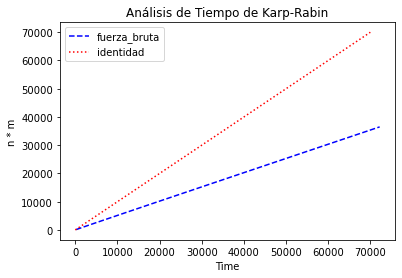
\includegraphics[width=0.5\textwidth]{../codigoPythonJupyter/rk/Final.png}
    \caption{Karp-Rabin (Anexo rabinkarp.ipynb)}
    \label{fig:kr}
\end{figure}


\section*{Comparación de todos}


% para probar que BM no es tan bueno para datos pequeños https://stackoverflow.com/questions/24806753/knuth-morris-pratt-vs-boyer-moore-binary-alphabet-vs-alphabet-with-large-numbe 
\begin{figure} [H]
    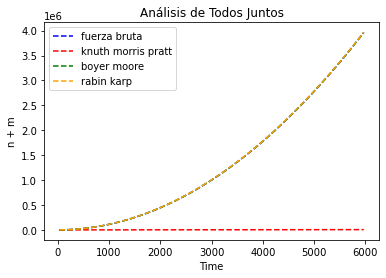
\includegraphics[width=0.5\textwidth]{../codigoPythonJupyter/Todos.png}
    \caption{Todos los algoritmos comparados (ver Anexo todos.ipynb)}
    \label{fig:all}
\end{figure}

Con esto podemos concluir que poniendo todos los algoritmos en el peor de los casos (todos los caracteres iguales) el kmp es el más eficiente.

Además decidimos probar los tres con un texto grande (buscar "Harry" dentro del primer libro de Harry Potter) y correrlo con el timeit de Python: (ver Anexo de pruebas.ipynb para más info)
\begin{table} [H]
    \begin{tabular}{| c | c | c | c |}
        \hline
        Fuerza Bruta & Knuth-Morris-Pratt & Boyer-Moore & Karp-Rabin \\
        \hline
        92.39191730198218 s & 93.05609979297151 s & 138.52656350799953 s & 170.72219764100737 s \\
        \hline
    \end{tabular}
    \caption{Harry Potter 1 buscando Harry}
    \label{tab:hp}
\end{table}


\phantomsection
\part*{ADN}% -capitulo de string matching con ejemplos ilustrativos propios
% \addcontentsline{toc}{part}{String Matching}

\phantomsection
\section*{Importancia del String Matching con el ADN}
\addcontentsline{toc}{section}{Importancia del String Matching con el ADN}

\quad El Ácido desoxirribonucleico o ADN es un ácido nucleico compuesto de 4 nucleótidos, estos son la adenina (A), timina (T), guanina (G) y citosina (C), además de estos 4 nucleótidos, existe un 5 que es el uracilo (U), pero este se encuentra en el ARN reemplazando a la timina (T). Este contiene las instrucciones y la información genética usadas en el desarrollo y funcionamiento de todo ser vivo, incluyendo algunos virus, además, es el responsable de la herencia genética, como el color de ojos, el color de piel, el cabello y todo tipo de cosas que podemos heredar de nuestros padres o antepasados, sin embargo, también es responsable de heredar ciertas enfermedades genéticas, como por ejemplo, la fibrosis quística, la hemofilia, la enfermedad de Huntington, etc. \\

\quad Con esto se buscar una base nitrogenada específica, hicimos pruebas con los cuatro algoritmos con una secuencia de ADN aleatoria generada en \href{http://www.faculty.ucr.edu/~mmaduro/random.htm}{este sitio}, y le corrimos con timeit.repeat() 
\begin{tabular}{|c|c|c|c|}

\end{tabular}

\quad Para efectos de esta investigación, hemos decidido utilizar la enfermedad de Huntington como ejemplo de string matching en una cadena de ADN. \\

\quad La enfermedad de Huntington es una enfermedad hereditaria que da la instrucción al cuerpo de producir una proteína llamada Huntingtina(HTT). Aunque se desconoce la función de dicha proteína, se cree que juega un papel importante en las neuronas. Esta enfermedad es provocada por una mutación en un segmento del ADN conocido como una repetición del trinucleótido CAG (citosina, adenina y guanina). Este segmento CAG normalmente se repite de 10 a 35 veces en personas sanas, sin embargo, en personas con la enfermedad de Huntington, dicho segmento se repite de 36 a as de 120 veces. \\

Como se puede ver en la siguiente imagen: 
\begin{figure} [H]
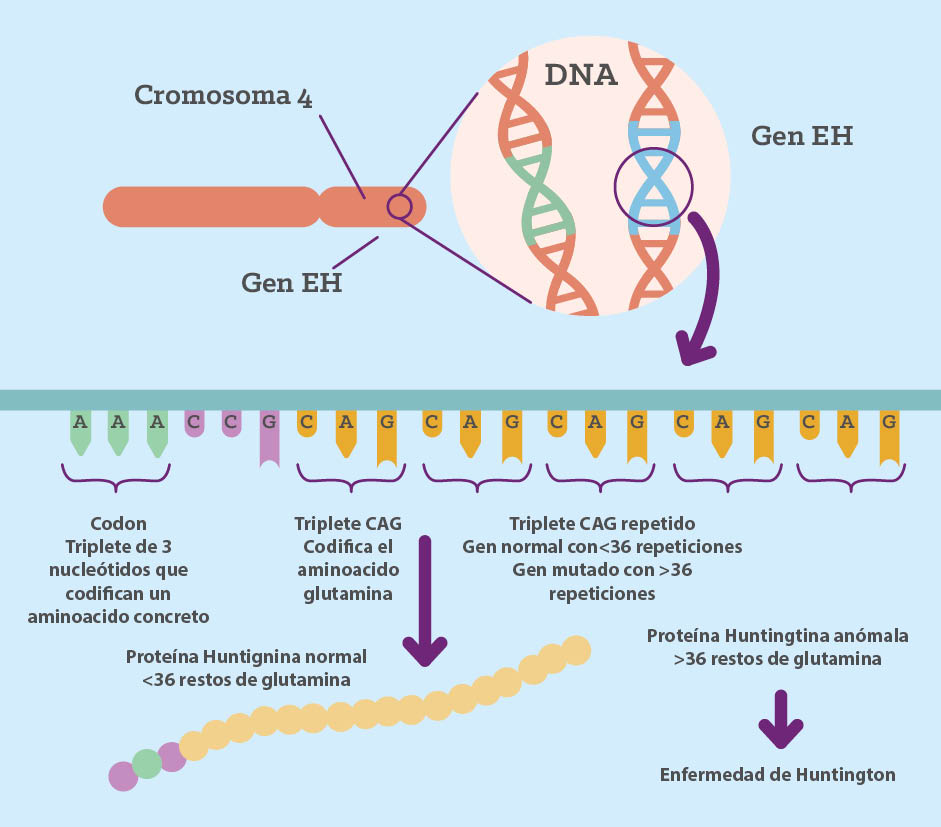
\includegraphics[width=1.0\textwidth]{causas-enfermedad-huntington.jpg}
\caption{Causes de Huntington}
\label{fig:Hunttington}
\end{figure}


\quad Para efectos del string matching, vamos a comprobar cuantas veces se repite  el segmento CAG en la cadena de ADN para comprobar si una persona padece de esta enfermedad.



% https://biolinksperu.com/blog/enfermedades-hereditarias-comunes/
% https://rochepacientes.es/enfermedad-huntington/causas.html

%-----------------------------------------------------------------------------------------------------------------------------------------------------
\phantomsection
\section*{Conclusión}
% \addcontentsline{toc}{section}{Conclusión}
\quad De esta investigación aprendimos, investigamos, estudiamos e intentamos entender lo mejor posible sobre algunos de los algoritmos de string matching existentes. Se profundizó sobre definiciones y se explicaron los 4 algoritmos solicitados. Hicimos análisis de tiempo de los algoritmos y aprendimos acerca de la prueba experimental en el campo de la informática. Se habló sobre el ADN y la enfermedad de Huntington y se aplicó un ejemplo sobre dicha enfermedad para probar los algoritmos. Aprendimos sobre la importancia que pueden tener los algoritmos de string matching en la vida cotidiana, tanto en algo tan complejo como detectar enfermedades en cadenas de ADN como algo tan simple como buscar una palabra en un texto. En el proceso aprendimos más sobre diferentes conceptos relacionados con string matching, aprendimos más sobre Python y sobre los algoritmos solicitados. Creamos implementaciones de dichos algoritmos utilizando diferentes fuentes y seudocódigos e intentamos darles distintos toques personales. Sin embargo, consideramos que aun tenemos un largo camino por recorrer dado que algunos de los datos “teóricos” fueron muy diferentes a los prácticos, pero igualmente le dedicamos mucho esfuerzo..

%----------------------------------------------------------------------------------------------------------------------------------------------------------------
\appendix


\newpage
% Referencias
\renewcommand\refname{\large\textbf{Referencias}}
\bibliography{ref}
\end{singlespace}
\end{document}